\documentclass{article}

\usepackage{noweb}
\noweboptions{smallcode,longchunks}

\usepackage[a4paper,margin=1in]{geometry}

\usepackage{colortbl}
\usepackage[colorlinks=true]{hyperref}
\usepackage{tikz}

% Define a handy paragraph opener
\newcommand{\hi}[1]{\noindent {\bf #1}}

% Remove noweb page break penalty
\def\nwendcode{\endtrivlist \endgroup}
\let\nwdocspar=\par

\title{Jargo Client\footnote{\url{https://github.com/jargors/Client}}}
\author{James J. Pan\\
  \small{\href{mailto:jamesjpan@outlook.com}{jamesjpan@outlook.com}}
}

\begin{document}
\maketitle
\pagestyle{noweb}

\tableofcontents

\section{Introduction}
\label{sec:introduction}
We supply an abstract base class for developing Jargo client ridesharing
algorithms. The class provides a standard interface for interacting with the
simulation engine (Figure~\ref{fig:client}). Algorithm developers extend the
base class to add specific customer-to-vehicle matching and vehicle routing
functionality.
The base class is developed using the
Noweb\footnote{\url{https://www.cs.tufts.edu/~nr/noweb/}} literate
programming\footnote{\url{http://literateprogramming.com/}} tool.  This file
({\tt{}src/JargoClient.nw}) is the source for both the documentation
({\tt{}doc/JargoClient.tex}) and the Java code (JargoClient.java)\footnote{See the
{\tt{}Makefile} for build details.}.

\begin{figure}[h]
\centering
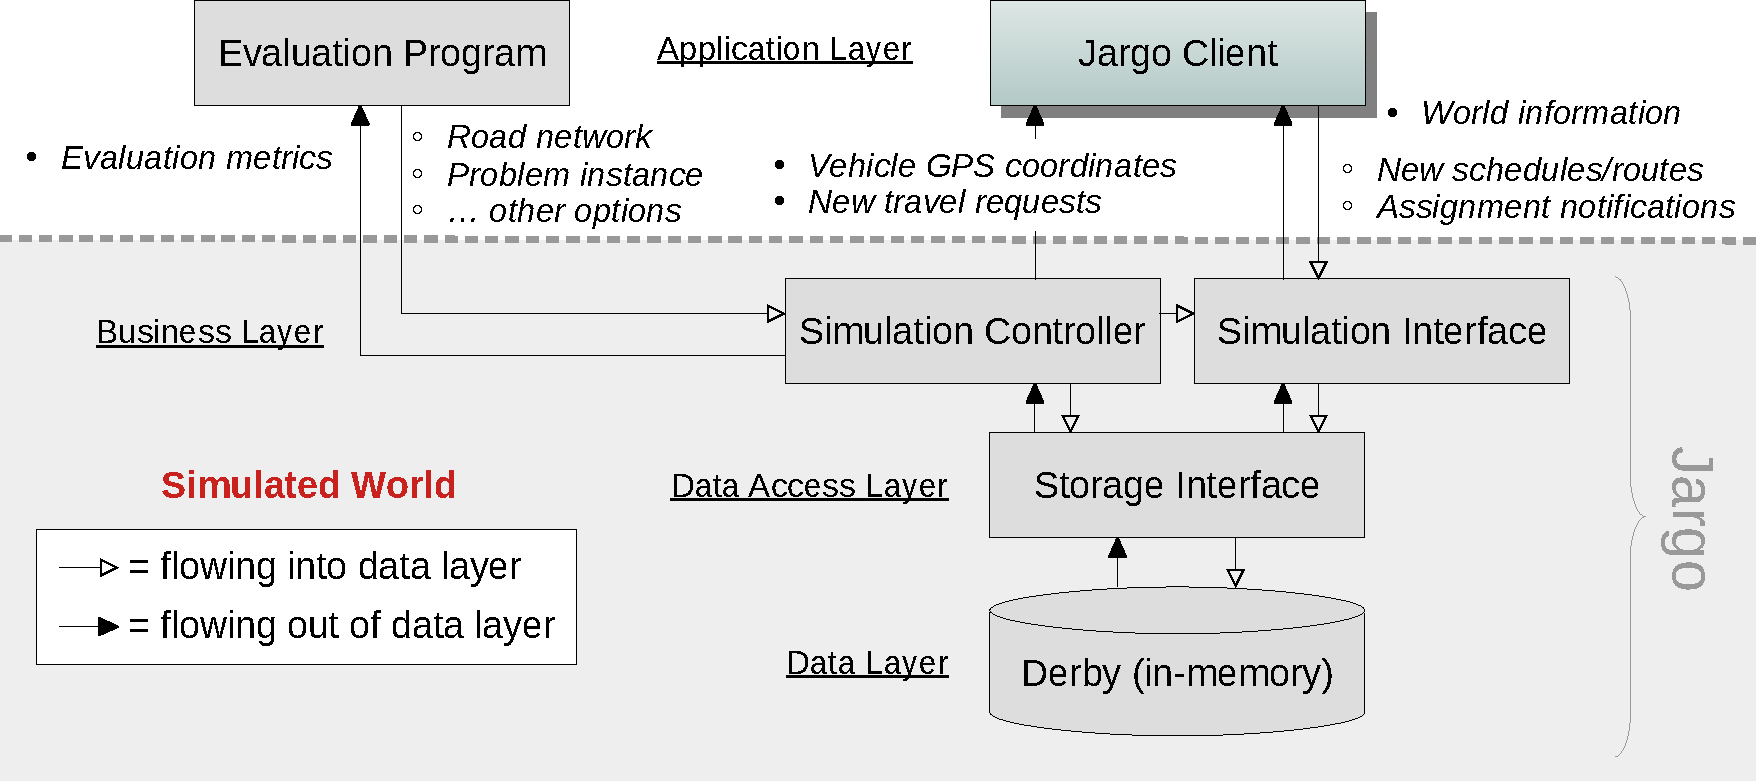
\includegraphics[width=150mm]{src/fig/client-fig}
\caption{Client within the Jargo stack.}
\label{fig:client}
\end{figure}

\section{Implementation Overview}
\nwfilename{src/JargoClient.nw}\nwbegincode{1}\sublabel{NW6iDVp-4V3s04-1}\nwmargintag{{\nwtagstyle{}\subpageref{NW6iDVp-4V3s04-1}}}\moddef{JargoClient.java~{\nwtagstyle{}\subpageref{NW6iDVp-4V3s04-1}}}\endmoddef\nwnotused{JargoClient.java}
  \LA{}JargoClient.java preamble~{\nwtagstyle{}\subpageref{NW6iDVp-Lginr-1}}\RA{}
  \LA{}\code{}JargoClient\edoc{} definition~{\nwtagstyle{}\subpageref{NW6iDVp-4CdRs3-1}}\RA{}
\nwendcode{}\nwbegindocs{2}\nwdocspar

\subsection{Preamble}
The preamble declares the package and imports dependencies.
\nwenddocs{}\nwbegincode{3}\sublabel{NW6iDVp-Lginr-1}\nwmargintag{{\nwtagstyle{}\subpageref{NW6iDVp-Lginr-1}}}\moddef{JargoClient.java preamble~{\nwtagstyle{}\subpageref{NW6iDVp-Lginr-1}}}\endmoddef\nwalsodefined{\\{NW6iDVp-Lginr-2}}\nwused{\\{NW6iDVp-4V3s04-1}}
package com.github.jargors;
\nwendcode{}\nwbegindocs{4}\nwdocspar
We import {\tt{}SimulationInterface} so we can interact with the simulated world,
and we import {\tt{}LocalDateTime} so we can query the physical time for
logging purposes.
\nwenddocs{}\nwbegincode{5}\sublabel{NW6iDVp-Lginr-2}\nwmargintag{{\nwtagstyle{}\subpageref{NW6iDVp-Lginr-2}}}\moddef{JargoClient.java preamble~{\nwtagstyle{}\subpageref{NW6iDVp-Lginr-1}}}\plusendmoddef
import com.github.jargors.SimulationInterface;
import com.github.jargors.DistanceUtilities;
import java.util.function.Supplier;
import java.time.LocalDateTime;
\nwendcode{}\nwbegindocs{6}\nwdocspar

\subsection{Class Definition}
The {\tt{}JargoClient} class consists of member variables, a constructor, and
public and protected methods. Note the {\tt{}abstract} keyword indicates the class
cannot be used directly.
\nwenddocs{}\nwbegincode{7}\sublabel{NW6iDVp-4CdRs3-1}\nwmargintag{{\nwtagstyle{}\subpageref{NW6iDVp-4CdRs3-1}}}\moddef{\code{}JargoClient\edoc{} definition~{\nwtagstyle{}\subpageref{NW6iDVp-4CdRs3-1}}}\endmoddef\nwused{\\{NW6iDVp-4V3s04-1}}
public abstract class JargoClient \{
  \LA{}\code{}JargoClient\edoc{} member variables~{\nwtagstyle{}\subpageref{NW6iDVp-zj3dK-1}}\RA{}
  \LA{}\code{}JargoClient\edoc{} constructor~{\nwtagstyle{}\subpageref{NW6iDVp-Ycmvi-1}}\RA{}
  \LA{}\code{}JargoClient\edoc{} public methods~{\nwtagstyle{}\subpageref{NW6iDVp-1eOdh6-1}}\RA{}
  \LA{}\code{}JargoClient\edoc{} protected methods~{\nwtagstyle{}\subpageref{NW6iDVp-HkhsI-1}}\RA{}
\}
\nwendcode{}\nwbegindocs{8}\nwdocspar

\subsection{Member Variables}
We define two containers for requests and server locations obtained from the
simulation engine. We also define the collection periods, in seconds. By
default, requests and server locations are collected every second.
\nwenddocs{}\nwbegincode{9}\sublabel{NW6iDVp-zj3dK-1}\nwmargintag{{\nwtagstyle{}\subpageref{NW6iDVp-zj3dK-1}}}\moddef{\code{}JargoClient\edoc{} member variables~{\nwtagstyle{}\subpageref{NW6iDVp-zj3dK-1}}}\endmoddef\nwused{\\{NW6iDVp-4CdRs3-1}}
protected int[] requests;
protected int[] locations;
protected int r_collection_period = 1;
protected int s_collection_period = 10;
protected SimulationInterface simulator;
protected DistanceUtilities distance = new DistanceUtilities();
\nwindexdefn{requests}{requests}{NW6iDVp-zj3dK-1}\nwindexdefn{locations}{locations}{NW6iDVp-zj3dK-1}\nwindexdefn{r{\char95}collection{\char95}period}{r:uncollection:unperiod}{NW6iDVp-zj3dK-1}\nwindexdefn{s{\char95}collection{\char95}period}{s:uncollection:unperiod}{NW6iDVp-zj3dK-1}\nwindexdefn{simulator}{simulator}{NW6iDVp-zj3dK-1}\nwindexdefn{distance}{distance}{NW6iDVp-zj3dK-1}\eatline
\nwidentdefs{\\{{distance}{distance}}\\{{locations}{locations}}\\{{r{\char95}collection{\char95}period}{r:uncollection:unperiod}}\\{{requests}{requests}}\\{{s{\char95}collection{\char95}period}{s:uncollection:unperiod}}\\{{simulator}{simulator}}}\nwendcode{}\nwbegindocs{10}\nwdocspar
\subsection{Constructor}
An actual algorithm might override the default constructor to perform
preprocessing tasks such as building a road network index.
\nwenddocs{}\nwbegincode{11}\sublabel{NW6iDVp-Ycmvi-1}\nwmargintag{{\nwtagstyle{}\subpageref{NW6iDVp-Ycmvi-1}}}\moddef{\code{}JargoClient\edoc{} constructor~{\nwtagstyle{}\subpageref{NW6iDVp-Ycmvi-1}}}\endmoddef\nwused{\\{NW6iDVp-4CdRs3-1}}
public JargoClient() \{ \}
\nwendcode{}\nwbegindocs{12}\nwdocspar

\section{Public Methods}
\nwenddocs{}\nwbegincode{13}\sublabel{NW6iDVp-1eOdh6-1}\nwmargintag{{\nwtagstyle{}\subpageref{NW6iDVp-1eOdh6-1}}}\moddef{\code{}JargoClient\edoc{} public methods~{\nwtagstyle{}\subpageref{NW6iDVp-1eOdh6-1}}}\endmoddef\nwused{\\{NW6iDVp-4CdRs3-1}}
  \LA{}Collect requests~{\nwtagstyle{}\subpageref{NW6iDVp-3Db6qU-1}}\RA{}
  \LA{}Collect server locations~{\nwtagstyle{}\subpageref{NW6iDVp-wbUkp-1}}\RA{}
  \LA{}Set simulation interface~{\nwtagstyle{}\subpageref{NW6iDVp-4etKpU-1}}\RA{}
  \LA{}Get/set request collection period~{\nwtagstyle{}\subpageref{NW6iDVp-4fmrsw-1}}\RA{}
  \LA{}Get/set server location collection period~{\nwtagstyle{}\subpageref{NW6iDVp-DxGq5-1}}\RA{}
  \LA{}Compute haversine~{\nwtagstyle{}\subpageref{NW6iDVp-1XfngC-1}}\RA{}
\nwendcode{}\nwbegindocs{14}\nwdocspar

\subsection{Obtaining Requests and Server Locations}
To obtain unassigned customer requests and server locations, we depend on
the simulation engine to push the data to the client. The {\tt{}\protect\nosublabel{NW6iDVp-1eOdh6-1-u6}\protect\nwindexuse{collectRequests}{collectRequests}{NW6iDVp-3Db6qU-1}collectRequests}(1)
and {\tt{}\protect\nwindexuse{collectServerLocations}{collectServerLocations}{NW6iDVp-wbUkp-1}collectServerLocations}(1) methods simply copy {\tt{}src} into
the client's working memory.

\subsubsection{{\tt{}\protect\nwindexuse{collectRequests}{collectRequests}{NW6iDVp-3Db6qU-1}collectRequests}(1)}
Array {\tt{}src} =

\noindent
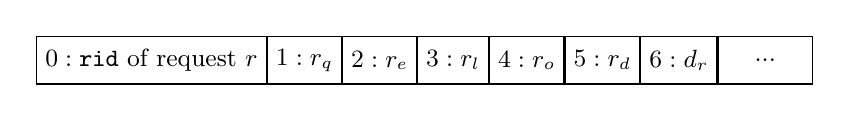
\begin{tikzpicture}
\small
\matrix[nodes={draw,minimum size=6mm}] {
  \node {$0:\textrm{{\tt{}rid} of request }r$};
 &\node {$1:r_q$}; & \node {$2:r_e$}; & \node {$3:r_l$};
 &\node {$4:r_o$}; & \node {$5:r_d$}; & \node {$6:d_r$};
 &\node[minimum width=12mm] {...};\\
};
\end{tikzpicture}

\noindent containing all $r$ queued to be assigned\footnote{See
\url{https://github.com/jargors/Storage} to learn about Jargo's data model.}.
After copying {\tt{}src} into {\tt{}\protect\nwindexuse{requests}{requests}{NW6iDVp-zj3dK-1}requests}, the {\tt{}\protect\nwindexuse{endCollectRequests}{endCollectRequests}{NW6iDVp-2fY8iU-1}endCollectRequests}(0) method
is executed.
\nwenddocs{}\nwbegincode{15}\sublabel{NW6iDVp-3Db6qU-1}\nwmargintag{{\nwtagstyle{}\subpageref{NW6iDVp-3Db6qU-1}}}\moddef{Collect requests~{\nwtagstyle{}\subpageref{NW6iDVp-3Db6qU-1}}}\endmoddef\nwused{\\{NW6iDVp-1eOdh6-1}}
public void collectRequests(int[] src) \{
  // Print("JargoClient collectRequests(1) got src of size "+src.length);
  requests = src.clone();
  endCollectRequests();
\}
\nwindexdefn{collectRequests}{collectRequests}{NW6iDVp-3Db6qU-1}\eatline
\nwidentdefs{\\{{collectRequests}{collectRequests}}}\nwidentuses{\\{{endCollectRequests}{endCollectRequests}}\\{{Print}{Print}}\\{{requests}{requests}}}\nwindexuse{endCollectRequests}{endCollectRequests}{NW6iDVp-3Db6qU-1}\nwindexuse{Print}{Print}{NW6iDVp-3Db6qU-1}\nwindexuse{requests}{requests}{NW6iDVp-3Db6qU-1}\nwendcode{}\nwbegindocs{16}\nwdocspar
\subsubsection{{\tt{}\protect\nwindexuse{collectServerLocations}{collectServerLocations}{NW6iDVp-wbUkp-1}collectServerLocations}(1)}
Array {\tt{}src} =

\noindent
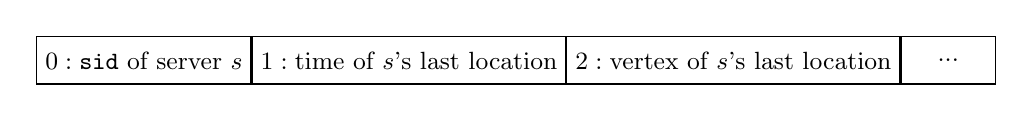
\begin{tikzpicture}
\small
\matrix[nodes={draw,minimum size=6mm}] {
  \node {$0:\textrm{{\tt{}sid} of server }s$};
 &\node {$1:\textrm{time of $s$'s last location}$};
 &\node {$2:\textrm{vertex of $s$'s last location}$};
 &\node[minimum width=12mm] {...};\\
};
\end{tikzpicture}

\noindent If locations are polled for and stored into {\tt{}src} at $t'$ world
time, then formally the last location for server $s$ is defined as waypoint
$(t,v)$ that satisfies $t=\textrm{argmin}_{(t,v)\in w_{\leq t'}} (t-t')$, where
$w_{\leq t'}$ is the server's traveled route.  In other words the last location
is the waypoint in the server's traveled route that is nearest $t'$.  After
copying {\tt{}src} into {\tt{}\protect\nwindexuse{locations}{locations}{NW6iDVp-zj3dK-1}locations}, the {\tt{}\protect\nwindexuse{endCollectServerLocations}{endCollectServerLocations}{NW6iDVp-2d6rGZ-1}endCollectServerLocations}(0) method
is executed.
\nwenddocs{}\nwbegincode{17}\sublabel{NW6iDVp-wbUkp-1}\nwmargintag{{\nwtagstyle{}\subpageref{NW6iDVp-wbUkp-1}}}\moddef{Collect server locations~{\nwtagstyle{}\subpageref{NW6iDVp-wbUkp-1}}}\endmoddef\nwused{\\{NW6iDVp-1eOdh6-1}}
public void collectServerLocations(int[] src) \{
  // Print("JargoClient collectServerLocations(1) got src of size "+src.length);
  locations = src.clone();
  endCollectServerLocations();
\}
\nwindexdefn{collectServerLocations}{collectServerLocations}{NW6iDVp-wbUkp-1}\eatline
\nwidentdefs{\\{{collectServerLocations}{collectServerLocations}}}\nwidentuses{\\{{endCollectServerLocations}{endCollectServerLocations}}\\{{locations}{locations}}\\{{Print}{Print}}}\nwindexuse{endCollectServerLocations}{endCollectServerLocations}{NW6iDVp-wbUkp-1}\nwindexuse{locations}{locations}{NW6iDVp-wbUkp-1}\nwindexuse{Print}{Print}{NW6iDVp-wbUkp-1}\nwendcode{}\nwbegindocs{18}\nwdocspar
\subsection{Getters and Setters}

\subsubsection{{\tt{}\protect\nwindexuse{setSimulationInterface}{setSimulationInterface}{NW6iDVp-4etKpU-1}setSimulationInterface}(1)}
\nwenddocs{}\nwbegincode{19}\sublabel{NW6iDVp-4etKpU-1}\nwmargintag{{\nwtagstyle{}\subpageref{NW6iDVp-4etKpU-1}}}\moddef{Set simulation interface~{\nwtagstyle{}\subpageref{NW6iDVp-4etKpU-1}}}\endmoddef\nwused{\\{NW6iDVp-1eOdh6-1}}
public void setSimulationInterface(SimulationInterface src) \{
  simulator = src;
  // Print("JargoClient setSimulationInterface(1)");
\}
\nwindexdefn{setSimulationInterface}{setSimulationInterface}{NW6iDVp-4etKpU-1}\eatline
\nwidentdefs{\\{{setSimulationInterface}{setSimulationInterface}}}\nwidentuses{\\{{Print}{Print}}\\{{simulator}{simulator}}}\nwindexuse{Print}{Print}{NW6iDVp-4etKpU-1}\nwindexuse{simulator}{simulator}{NW6iDVp-4etKpU-1}\nwendcode{}\nwbegindocs{20}\nwdocspar
\subsubsection{{\tt{}\protect\nwindexuse{getRequestCollectionPeriod}{getRequestCollectionPeriod}{NW6iDVp-4fmrsw-1}getRequestCollectionPeriod}(0)}
\nwenddocs{}\nwbegincode{21}\sublabel{NW6iDVp-4fmrsw-1}\nwmargintag{{\nwtagstyle{}\subpageref{NW6iDVp-4fmrsw-1}}}\moddef{Get/set request collection period~{\nwtagstyle{}\subpageref{NW6iDVp-4fmrsw-1}}}\endmoddef\nwalsodefined{\\{NW6iDVp-4fmrsw-2}}\nwused{\\{NW6iDVp-1eOdh6-1}}
public int getRequestCollectionPeriod() \{
  return r_collection_period;
\}
\nwindexdefn{getRequestCollectionPeriod}{getRequestCollectionPeriod}{NW6iDVp-4fmrsw-1}\eatline
\nwidentdefs{\\{{getRequestCollectionPeriod}{getRequestCollectionPeriod}}}\nwidentuses{\\{{r{\char95}collection{\char95}period}{r:uncollection:unperiod}}}\nwindexuse{r{\char95}collection{\char95}period}{r:uncollection:unperiod}{NW6iDVp-4fmrsw-1}\nwendcode{}\nwbegindocs{22}\nwdocspar
\subsubsection{{\tt{}\protect\nwindexuse{setRequestCollectionPeriod}{setRequestCollectionPeriod}{NW6iDVp-4fmrsw-2}setRequestCollectionPeriod}(1)}
\nwenddocs{}\nwbegincode{23}\sublabel{NW6iDVp-4fmrsw-2}\nwmargintag{{\nwtagstyle{}\subpageref{NW6iDVp-4fmrsw-2}}}\moddef{Get/set request collection period~{\nwtagstyle{}\subpageref{NW6iDVp-4fmrsw-1}}}\plusendmoddef
public void setRequestCollectionPeriod(int t) \{
  r_collection_period = t;
\}
\nwindexdefn{setRequestCollectionPeriod}{setRequestCollectionPeriod}{NW6iDVp-4fmrsw-2}\eatline
\nwidentdefs{\\{{setRequestCollectionPeriod}{setRequestCollectionPeriod}}}\nwidentuses{\\{{r{\char95}collection{\char95}period}{r:uncollection:unperiod}}}\nwindexuse{r{\char95}collection{\char95}period}{r:uncollection:unperiod}{NW6iDVp-4fmrsw-2}\nwendcode{}\nwbegindocs{24}\nwdocspar
\subsubsection{{\tt{}\protect\nwindexuse{getServerLocationCollectionPeriod}{getServerLocationCollectionPeriod}{NW6iDVp-DxGq5-1}getServerLocationCollectionPeriod}(0)}
\nwenddocs{}\nwbegincode{25}\sublabel{NW6iDVp-DxGq5-1}\nwmargintag{{\nwtagstyle{}\subpageref{NW6iDVp-DxGq5-1}}}\moddef{Get/set server location collection period~{\nwtagstyle{}\subpageref{NW6iDVp-DxGq5-1}}}\endmoddef\nwalsodefined{\\{NW6iDVp-DxGq5-2}}\nwused{\\{NW6iDVp-1eOdh6-1}}
public int getServerLocationCollectionPeriod () \{
  return s_collection_period;
\}
\nwindexdefn{getServerLocationCollectionPeriod}{getServerLocationCollectionPeriod}{NW6iDVp-DxGq5-1}\eatline
\nwidentdefs{\\{{getServerLocationCollectionPeriod}{getServerLocationCollectionPeriod}}}\nwidentuses{\\{{s{\char95}collection{\char95}period}{s:uncollection:unperiod}}}\nwindexuse{s{\char95}collection{\char95}period}{s:uncollection:unperiod}{NW6iDVp-DxGq5-1}\nwendcode{}\nwbegindocs{26}\nwdocspar
\subsubsection{{\tt{}\protect\nwindexuse{setServerLocationCollectionPeriod}{setServerLocationCollectionPeriod}{NW6iDVp-DxGq5-2}setServerLocationCollectionPeriod}(1)}
\nwenddocs{}\nwbegincode{27}\sublabel{NW6iDVp-DxGq5-2}\nwmargintag{{\nwtagstyle{}\subpageref{NW6iDVp-DxGq5-2}}}\moddef{Get/set server location collection period~{\nwtagstyle{}\subpageref{NW6iDVp-DxGq5-1}}}\plusendmoddef
public void setServerLocationCollectionPeriod(int t) \{
  s_collection_period = t;
\}
\nwindexdefn{setServerLocationCollectionPeriod}{setServerLocationCollectionPeriod}{NW6iDVp-DxGq5-2}\eatline
\nwidentdefs{\\{{setServerLocationCollectionPeriod}{setServerLocationCollectionPeriod}}}\nwidentuses{\\{{s{\char95}collection{\char95}period}{s:uncollection:unperiod}}}\nwindexuse{s{\char95}collection{\char95}period}{s:uncollection:unperiod}{NW6iDVp-DxGq5-2}\nwendcode{}\nwbegindocs{28}\nwdocspar
\subsubsection{{\tt{}\protect\nwindexuse{computeHaversine}{computeHaversine}{NW6iDVp-1XfngC-1}computeHaversine}(2)}
\nwenddocs{}\nwbegincode{29}\sublabel{NW6iDVp-1XfngC-1}\nwmargintag{{\nwtagstyle{}\subpageref{NW6iDVp-1XfngC-1}}}\moddef{Compute haversine~{\nwtagstyle{}\subpageref{NW6iDVp-1XfngC-1}}}\endmoddef\nwused{\\{NW6iDVp-1eOdh6-1}}
public int computeHaversine(int u, int v) \{
  int[] U = simulator.queryVertex(u);
  int[] V = simulator.queryVertex(v);
  return distance.computeHaversine(U[0], U[1], V[0], V[1]);
\}
\nwindexdefn{computeHaversine}{computeHaversine}{NW6iDVp-1XfngC-1}\eatline
\nwidentdefs{\\{{computeHaversine}{computeHaversine}}}\nwidentuses{\\{{distance}{distance}}\\{{simulator}{simulator}}}\nwindexuse{distance}{distance}{NW6iDVp-1XfngC-1}\nwindexuse{simulator}{simulator}{NW6iDVp-1XfngC-1}\nwendcode{}\nwbegindocs{30}\nwdocspar
\section{Private Methods}
\nwenddocs{}\nwbegincode{31}\sublabel{NW6iDVp-HkhsI-1}\nwmargintag{{\nwtagstyle{}\subpageref{NW6iDVp-HkhsI-1}}}\moddef{\code{}JargoClient\edoc{} protected methods~{\nwtagstyle{}\subpageref{NW6iDVp-HkhsI-1}}}\endmoddef\nwused{\\{NW6iDVp-4CdRs3-1}}
  \LA{}End collect requests~{\nwtagstyle{}\subpageref{NW6iDVp-2fY8iU-1}}\RA{}
  \LA{}End collect server locations~{\nwtagstyle{}\subpageref{NW6iDVp-2d6rGZ-1}}\RA{}
  \LA{}Handle request~{\nwtagstyle{}\subpageref{NW6iDVp-2856ar-1}}\RA{}
  \LA{}Handle server location~{\nwtagstyle{}\subpageref{NW6iDVp-2xqRZA-1}}\RA{}
  \LA{}Print a message~{\nwtagstyle{}\subpageref{NW6iDVp-2wEn3G-1}}\RA{}

\nwendcode{}\nwbegindocs{32}\nwdocspar

\subsection{{\tt{}\protect\nosublabel{NW6iDVp-HkhsI-1-u5}\protect\nwindexuse{endCollectRequests}{endCollectRequests}{NW6iDVp-2fY8iU-1}endCollectRequests}(0)}
After requests are collected, {\tt{}\protect\nwindexuse{handleRequest}{handleRequest}{NW6iDVp-2856ar-1}handleRequest}(1) is executed on each one.
\nwenddocs{}\nwbegincode{33}\sublabel{NW6iDVp-2fY8iU-1}\nwmargintag{{\nwtagstyle{}\subpageref{NW6iDVp-2fY8iU-1}}}\moddef{End collect requests~{\nwtagstyle{}\subpageref{NW6iDVp-2fY8iU-1}}}\endmoddef\nwused{\\{NW6iDVp-HkhsI-1}}
protected void endCollectRequests() \{
  // Print("JargoClient endCollectRequests(0)");
  for (int i = 0; i < (requests.length - 6); i += 7) \{
    // Print("JargoClient endCollectRequests(0)->handleRequest(..) on i="+i);
    handleRequest(new int[] \{
      requests[i],
      requests[(i + 1)],
      requests[(i + 2)],
      requests[(i + 3)],
      requests[(i + 4)],
      requests[(i + 5)],
      requests[(i + 6)]
    \});
  \}
\}
\nwindexdefn{endCollectRequests}{endCollectRequests}{NW6iDVp-2fY8iU-1}\eatline
\nwidentdefs{\\{{endCollectRequests}{endCollectRequests}}}\nwidentuses{\\{{handleRequest}{handleRequest}}\\{{Print}{Print}}\\{{requests}{requests}}}\nwindexuse{handleRequest}{handleRequest}{NW6iDVp-2fY8iU-1}\nwindexuse{Print}{Print}{NW6iDVp-2fY8iU-1}\nwindexuse{requests}{requests}{NW6iDVp-2fY8iU-1}\nwendcode{}\nwbegindocs{34}\nwdocspar
\subsection{{\tt{}\protect\nwindexuse{endCollectServerLocations}{endCollectServerLocations}{NW6iDVp-2d6rGZ-1}endCollectServerLocations}(0)}
After server locations are collected, {\tt{}\protect\nwindexuse{handleServerLocation}{handleServerLocation}{NW6iDVp-2xqRZA-1}handleServerLocation}(1) is executed
on each one.
\nwenddocs{}\nwbegincode{35}\sublabel{NW6iDVp-2d6rGZ-1}\nwmargintag{{\nwtagstyle{}\subpageref{NW6iDVp-2d6rGZ-1}}}\moddef{End collect server locations~{\nwtagstyle{}\subpageref{NW6iDVp-2d6rGZ-1}}}\endmoddef\nwused{\\{NW6iDVp-HkhsI-1}}
protected void endCollectServerLocations() \{
  // Print("JargoClient endCollectServerLocations(0)");
  for (int i = 0; i < (locations.length - 2); i += 3) \{
    // Print("JargoClient endCollectServerLocations(0)->handleServerLocation(..) on i="+i);
    handleServerLocation(new int[] \{
      locations[i],
      locations[(i + 1)],
      locations[(i + 2)]
    \});
  \}
\}
\nwindexdefn{endCollectServerLocations}{endCollectServerLocations}{NW6iDVp-2d6rGZ-1}\eatline
\nwidentdefs{\\{{endCollectServerLocations}{endCollectServerLocations}}}\nwidentuses{\\{{handleServerLocation}{handleServerLocation}}\\{{locations}{locations}}\\{{Print}{Print}}}\nwindexuse{handleServerLocation}{handleServerLocation}{NW6iDVp-2d6rGZ-1}\nwindexuse{locations}{locations}{NW6iDVp-2d6rGZ-1}\nwindexuse{Print}{Print}{NW6iDVp-2d6rGZ-1}\nwendcode{}\nwbegindocs{36}\nwdocspar
\subsection{{\tt{}\protect\nwindexuse{handleRequest}{handleRequest}{NW6iDVp-2856ar-1}handleRequest}(1)}
Array {\tt{}r} =

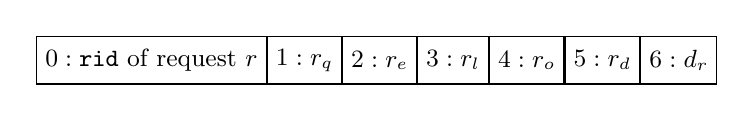
\begin{tikzpicture}
\small
\matrix[nodes={draw,minimum size=6mm}] {
  \node {$0:\textrm{{\tt{}rid} of request $r$}$};
 &\node {$1:r_q$}; & \node {$2:r_e$}; & \node {$3:r_l$};
 &\node {$4:r_o$}; & \node {$5:r_d$}; & \node {$6:d_r$};\\
};
\end{tikzpicture}

\noindent By default, {\tt{}\protect\nwindexuse{handleRequest}{handleRequest}{NW6iDVp-2856ar-1}handleRequest}(1) simply prints {\tt{}rid}.
\nwenddocs{}\nwbegincode{37}\sublabel{NW6iDVp-2856ar-1}\nwmargintag{{\nwtagstyle{}\subpageref{NW6iDVp-2856ar-1}}}\moddef{Handle request~{\nwtagstyle{}\subpageref{NW6iDVp-2856ar-1}}}\endmoddef\nwused{\\{NW6iDVp-HkhsI-1}}
protected void handleRequest(int[] r) \{
  // Print("JargoClient handleRequest(1) got Request "+r[0]);
\}
\nwindexdefn{handleRequest}{handleRequest}{NW6iDVp-2856ar-1}\eatline
\nwidentdefs{\\{{handleRequest}{handleRequest}}}\nwidentuses{\\{{Print}{Print}}}\nwindexuse{Print}{Print}{NW6iDVp-2856ar-1}\nwendcode{}\nwbegindocs{38}\nwdocspar
\subsection{{\tt{}\protect\nwindexuse{handleServerLocation}{handleServerLocation}{NW6iDVp-2xqRZA-1}handleServerLocation}(1)}
Array {\tt{}loc} =

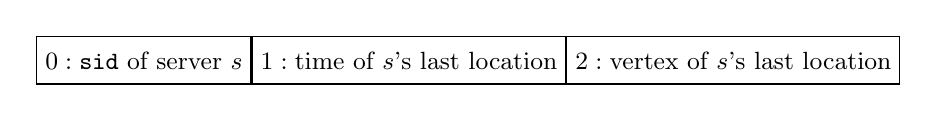
\begin{tikzpicture}
\small
\matrix[nodes={draw,minimum size=6mm}] {
  \node {$0:\textrm{{\tt{}sid} of server $s$}$};
 &\node {$1:\textrm{time of $s$'s last location}$};
 &\node {$2:\textrm{vertex of $s$'s last location}$};\\
};
\end{tikzpicture}

\noindent By default, {\tt{}\protect\nwindexuse{handleServerLocation}{handleServerLocation}{NW6iDVp-2xqRZA-1}handleServerLocation}(1) simply prints {\tt{}sid}.
\nwenddocs{}\nwbegincode{39}\sublabel{NW6iDVp-2xqRZA-1}\nwmargintag{{\nwtagstyle{}\subpageref{NW6iDVp-2xqRZA-1}}}\moddef{Handle server location~{\nwtagstyle{}\subpageref{NW6iDVp-2xqRZA-1}}}\endmoddef\nwused{\\{NW6iDVp-HkhsI-1}}
protected void handleServerLocation(int[] loc) \{
  // Print("JargoClient handleServerLocation(1) got Server "+loc[0]);
\}
\nwindexdefn{handleServerLocation}{handleServerLocation}{NW6iDVp-2xqRZA-1}\eatline
\nwidentdefs{\\{{handleServerLocation}{handleServerLocation}}}\nwidentuses{\\{{Print}{Print}}}\nwindexuse{Print}{Print}{NW6iDVp-2xqRZA-1}\nwendcode{}\nwbegindocs{40}\nwdocspar
\subsection{{\tt{}\protect\nwindexuse{Print}{Print}{NW6iDVp-2wEn3G-1}Print}(1)}
\nwenddocs{}\nwbegincode{41}\sublabel{NW6iDVp-2wEn3G-1}\nwmargintag{{\nwtagstyle{}\subpageref{NW6iDVp-2wEn3G-1}}}\moddef{Print a message~{\nwtagstyle{}\subpageref{NW6iDVp-2wEn3G-1}}}\endmoddef\nwused{\\{NW6iDVp-HkhsI-1}}
protected void Print(String msg) \{
  System.out.println("[JargoClient]["+LocalDateTime.now()+"]"
    + "[t="+simulator.getSimulationWorldTime()+"] "+msg);
\}
\nwindexdefn{Print}{Print}{NW6iDVp-2wEn3G-1}\eatline
\nwidentdefs{\\{{Print}{Print}}}\nwidentuses{\\{{simulator}{simulator}}}\nwindexuse{simulator}{simulator}{NW6iDVp-2wEn3G-1}\nwendcode{}

\nwixlogsorted{c}{{\code{}JargoClient\edoc{} constructor}{NW6iDVp-Ycmvi-1}{\nwixu{NW6iDVp-4CdRs3-1}\nwixd{NW6iDVp-Ycmvi-1}}}%
\nwixlogsorted{c}{{\code{}JargoClient\edoc{} definition}{NW6iDVp-4CdRs3-1}{\nwixu{NW6iDVp-4V3s04-1}\nwixd{NW6iDVp-4CdRs3-1}}}%
\nwixlogsorted{c}{{\code{}JargoClient\edoc{} member variables}{NW6iDVp-zj3dK-1}{\nwixu{NW6iDVp-4CdRs3-1}\nwixd{NW6iDVp-zj3dK-1}}}%
\nwixlogsorted{c}{{\code{}JargoClient\edoc{} protected methods}{NW6iDVp-HkhsI-1}{\nwixu{NW6iDVp-4CdRs3-1}\nwixd{NW6iDVp-HkhsI-1}}}%
\nwixlogsorted{c}{{\code{}JargoClient\edoc{} public methods}{NW6iDVp-1eOdh6-1}{\nwixu{NW6iDVp-4CdRs3-1}\nwixd{NW6iDVp-1eOdh6-1}}}%
\nwixlogsorted{c}{{Collect requests}{NW6iDVp-3Db6qU-1}{\nwixu{NW6iDVp-1eOdh6-1}\nwixd{NW6iDVp-3Db6qU-1}}}%
\nwixlogsorted{c}{{Collect server locations}{NW6iDVp-wbUkp-1}{\nwixu{NW6iDVp-1eOdh6-1}\nwixd{NW6iDVp-wbUkp-1}}}%
\nwixlogsorted{c}{{Compute haversine}{NW6iDVp-1XfngC-1}{\nwixu{NW6iDVp-1eOdh6-1}\nwixd{NW6iDVp-1XfngC-1}}}%
\nwixlogsorted{c}{{End collect requests}{NW6iDVp-2fY8iU-1}{\nwixu{NW6iDVp-HkhsI-1}\nwixd{NW6iDVp-2fY8iU-1}}}%
\nwixlogsorted{c}{{End collect server locations}{NW6iDVp-2d6rGZ-1}{\nwixu{NW6iDVp-HkhsI-1}\nwixd{NW6iDVp-2d6rGZ-1}}}%
\nwixlogsorted{c}{{Get/set request collection period}{NW6iDVp-4fmrsw-1}{\nwixu{NW6iDVp-1eOdh6-1}\nwixd{NW6iDVp-4fmrsw-1}\nwixd{NW6iDVp-4fmrsw-2}}}%
\nwixlogsorted{c}{{Get/set server location collection period}{NW6iDVp-DxGq5-1}{\nwixu{NW6iDVp-1eOdh6-1}\nwixd{NW6iDVp-DxGq5-1}\nwixd{NW6iDVp-DxGq5-2}}}%
\nwixlogsorted{c}{{Handle request}{NW6iDVp-2856ar-1}{\nwixu{NW6iDVp-HkhsI-1}\nwixd{NW6iDVp-2856ar-1}}}%
\nwixlogsorted{c}{{Handle server location}{NW6iDVp-2xqRZA-1}{\nwixu{NW6iDVp-HkhsI-1}\nwixd{NW6iDVp-2xqRZA-1}}}%
\nwixlogsorted{c}{{JargoClient.java}{NW6iDVp-4V3s04-1}{\nwixd{NW6iDVp-4V3s04-1}}}%
\nwixlogsorted{c}{{JargoClient.java preamble}{NW6iDVp-Lginr-1}{\nwixu{NW6iDVp-4V3s04-1}\nwixd{NW6iDVp-Lginr-1}\nwixd{NW6iDVp-Lginr-2}}}%
\nwixlogsorted{c}{{Print a message}{NW6iDVp-2wEn3G-1}{\nwixu{NW6iDVp-HkhsI-1}\nwixd{NW6iDVp-2wEn3G-1}}}%
\nwixlogsorted{c}{{Set simulation interface}{NW6iDVp-4etKpU-1}{\nwixu{NW6iDVp-1eOdh6-1}\nwixd{NW6iDVp-4etKpU-1}}}%
\nwixlogsorted{i}{{collectRequests}{collectRequests}}%
\nwixlogsorted{i}{{collectServerLocations}{collectServerLocations}}%
\nwixlogsorted{i}{{computeHaversine}{computeHaversine}}%
\nwixlogsorted{i}{{distance}{distance}}%
\nwixlogsorted{i}{{endCollectRequests}{endCollectRequests}}%
\nwixlogsorted{i}{{endCollectServerLocations}{endCollectServerLocations}}%
\nwixlogsorted{i}{{getRequestCollectionPeriod}{getRequestCollectionPeriod}}%
\nwixlogsorted{i}{{getServerLocationCollectionPeriod}{getServerLocationCollectionPeriod}}%
\nwixlogsorted{i}{{handleRequest}{handleRequest}}%
\nwixlogsorted{i}{{handleServerLocation}{handleServerLocation}}%
\nwixlogsorted{i}{{locations}{locations}}%
\nwixlogsorted{i}{{Print}{Print}}%
\nwixlogsorted{i}{{r{\char95}collection{\char95}period}{r:uncollection:unperiod}}%
\nwixlogsorted{i}{{requests}{requests}}%
\nwixlogsorted{i}{{s{\char95}collection{\char95}period}{s:uncollection:unperiod}}%
\nwixlogsorted{i}{{setRequestCollectionPeriod}{setRequestCollectionPeriod}}%
\nwixlogsorted{i}{{setServerLocationCollectionPeriod}{setServerLocationCollectionPeriod}}%
\nwixlogsorted{i}{{setSimulationInterface}{setSimulationInterface}}%
\nwixlogsorted{i}{{simulator}{simulator}}%
\nwbegindocs{42}\nwdocspar
\appendix

\section{Appendix: List of Chunks}
\label{ap:list-of-chunks}
\nowebchunks

\section{Appendix: List of Identifiers}
\label{ap:list-of-identifiers}
\nowebindex

\end{document}

\nwenddocs{}
